\begin{problem}
试描述SOAP包的结构,并结合该结构,阐述SOAP处理模型(无需准确给出相关命名空间和元素名称)
\end{problem}

\begin{solution}
\begin{figure}[H]
    \vspace{-0.5em}
	\centering
	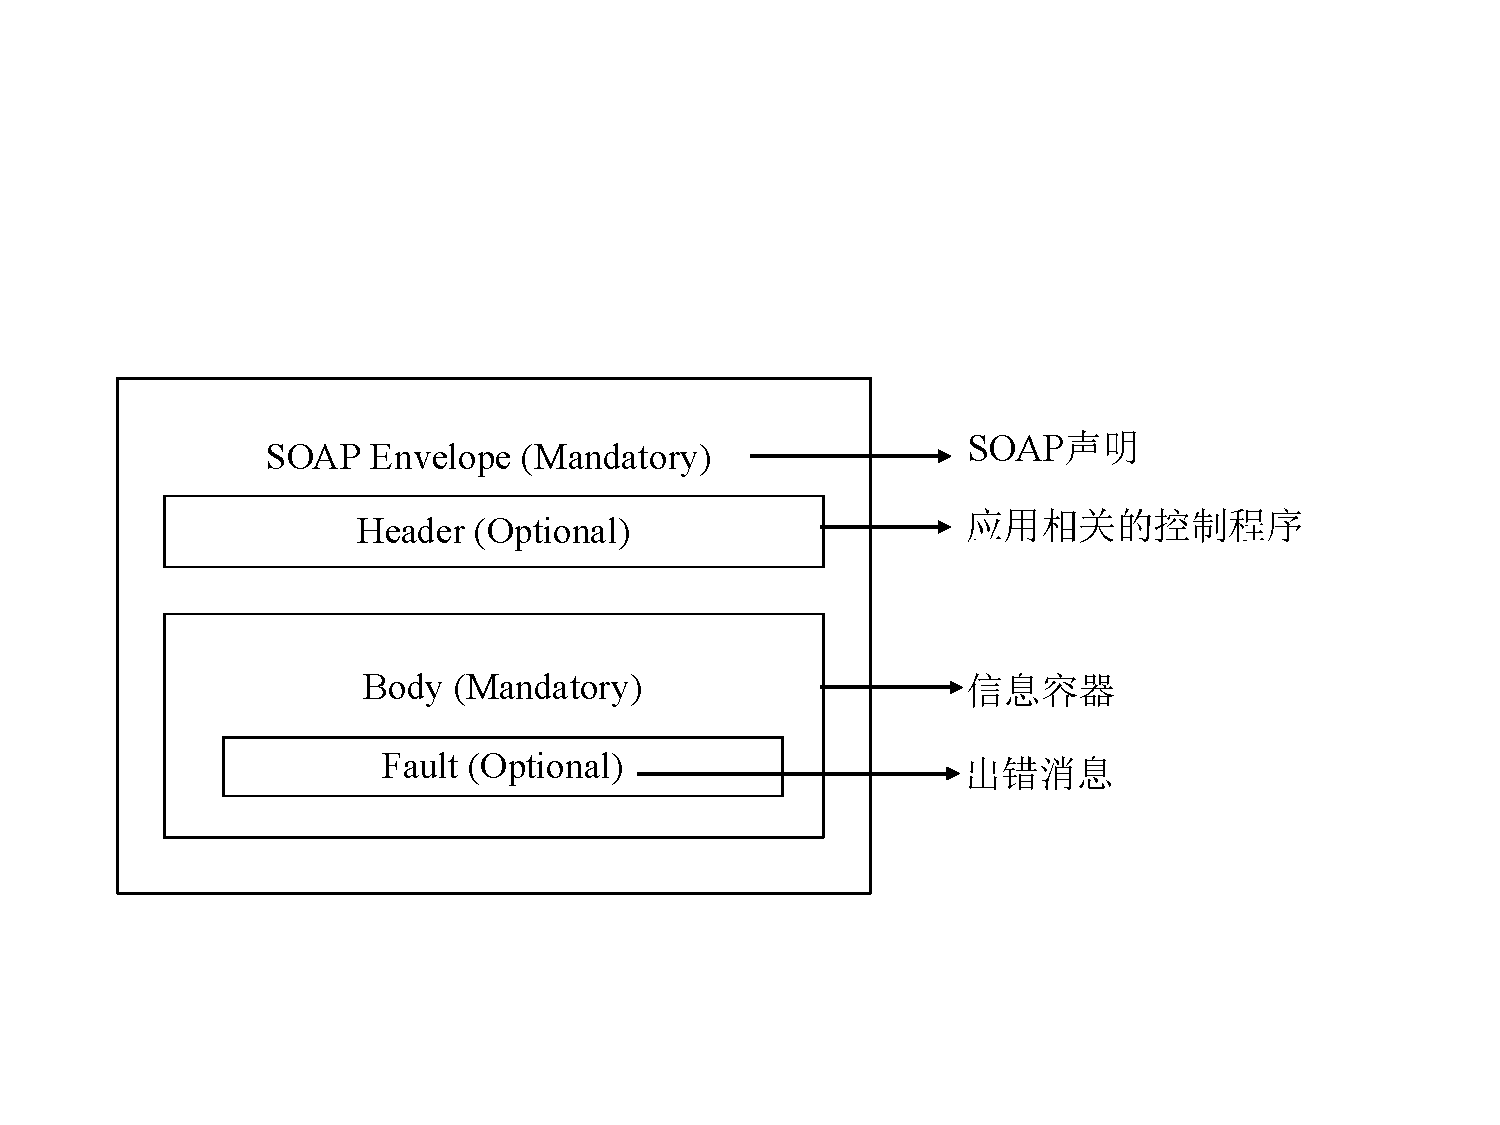
\includegraphics[width=0.65\textwidth]{SOAP结构.pdf}
    \vspace{-1em}
\end{figure}

SOAP包本质是一个XML文档,包含下列元素:
\begin{itemize}
    \item Envelope元素:必需元素,根元素,标识此XML文档为一条 SOAP 消息。可以包含命名空间和声明额外的属性。如果出现额外属性,则必须使用命名空间修饰。
    \item Header 元素:可选元素,有关 SOAP 消息的应用程序专用信息(比如认证、支付等)。
    \item Body 元素:必需元素,包含所有的调用和响应信息。
    \item Fault 元素:可选元素,提供有关在处理此消息所发生错误的信息。
\end{itemize}

SOAP处理模型:
\begin{enumerate}[label=\arabic*.]
    \item 组装SOAP消息:发送方将要发送的数据按照SOAP消息格式进行组装。SOAP消息包括可选的Header和必需的body。
    \item 封装SOAP消息:发送方将组装好的SOAP消息封装成一个标准的HTTP POST请求,然后发送给接收方。封装时需要将SOAP消息体作为HTTP POST请求的请求体(RequestBody)来发送。
    \item 解析SOAP消息:接收方接收到HTTP POST请求后,将请求体中的SOAP消息体进行解析,并提取出其中的数据。
    \item 处理SOAP消息:接收方根据解析出的数据进行业务处理,然后将处理结果封装成SOAP消息格式,通过HTTP响应将处理结果发送回去。
\end{enumerate}

SOAP的两种使用方式:
\begin{figure}[H]
	\setcounter{subfigure}{0}
	\centering
	\vspace{-2em}	
	\subfloat[没有中间转发节点]{
	\begin{minipage}[t]{0.3\linewidth}
	\centering
	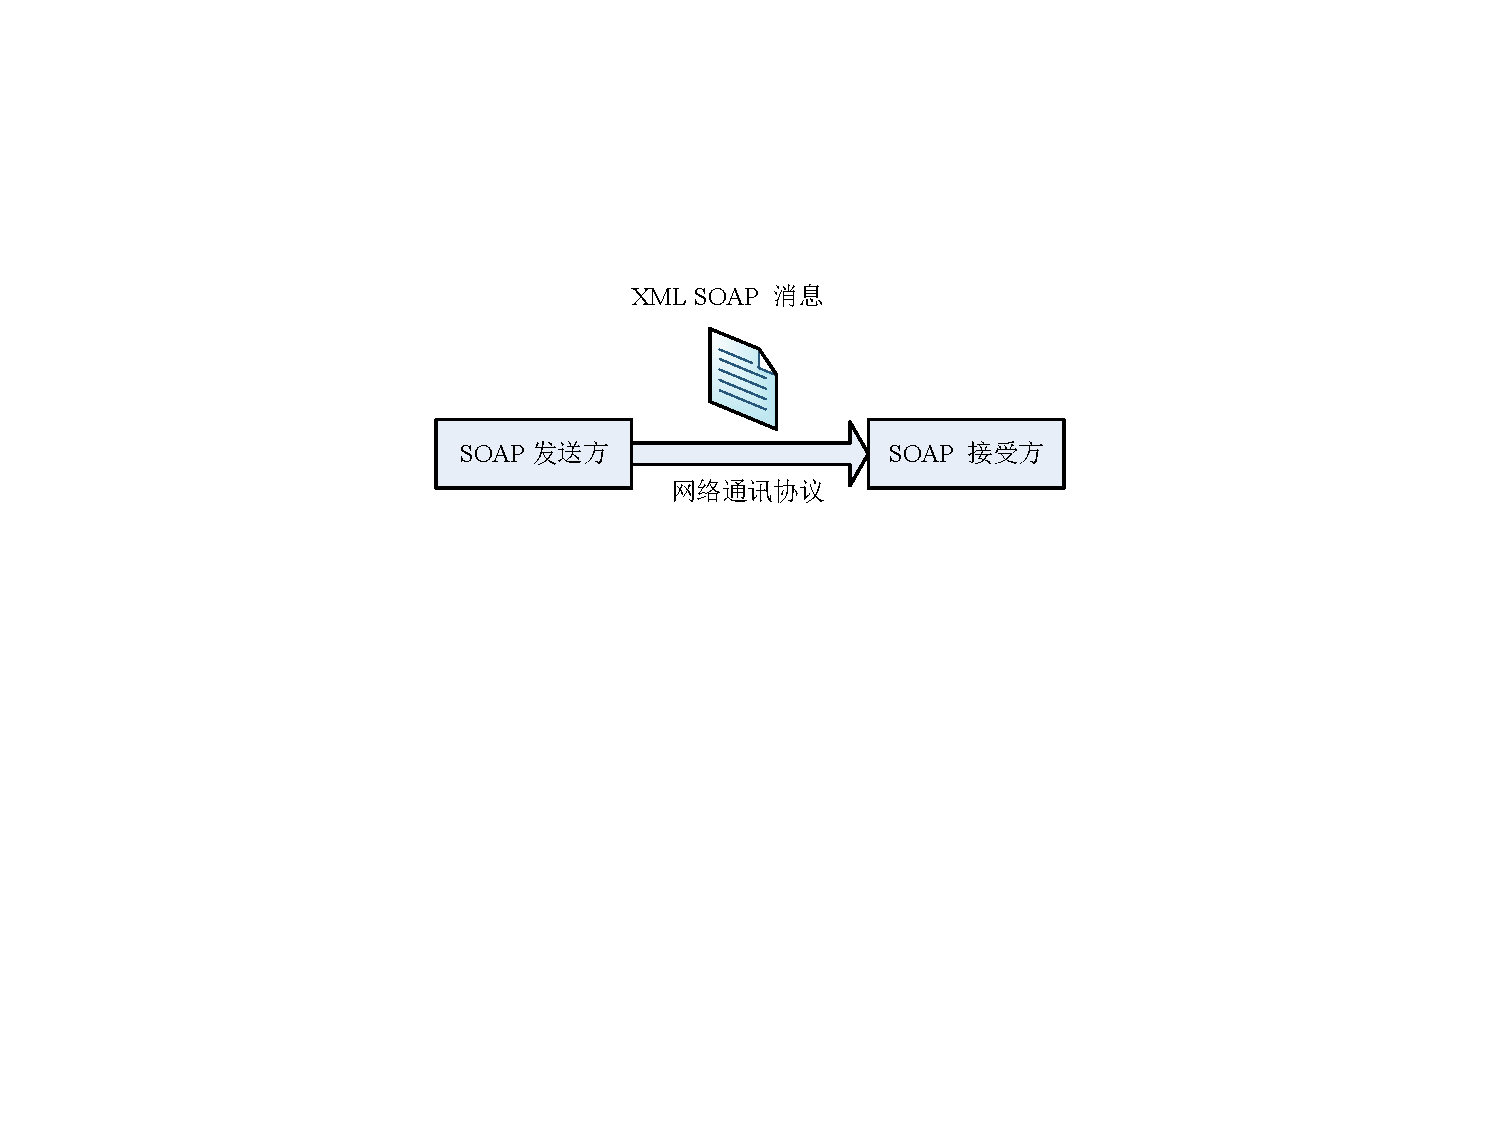
\includegraphics[width=0.97\linewidth]{SOAP没有中间转发节点.pdf}
	\end{minipage}
	}
    \subfloat[有多个中间转发节点]{
	\begin{minipage}[t]{0.66\linewidth}
	\centering
	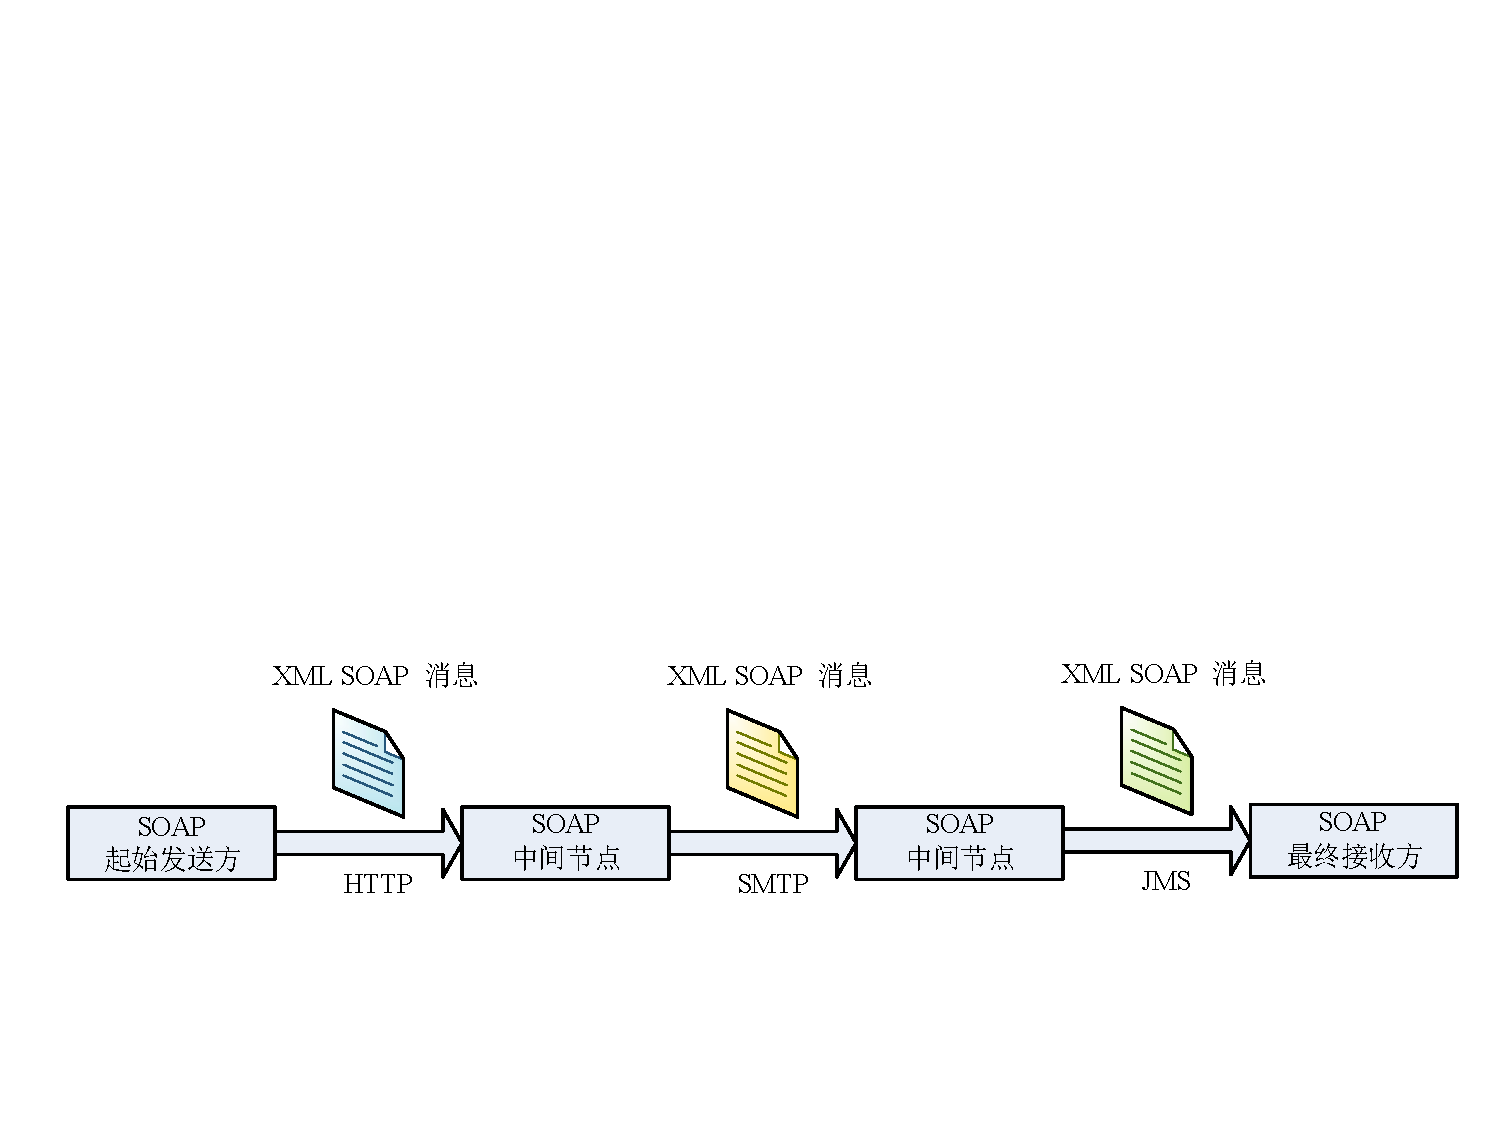
\includegraphics[width=0.93\linewidth]{SOAP有多个中间转发节点.pdf}
	\end{minipage}
	}
	\centering
	\vspace{-1.5em}
\end{figure}

SOAP的两种交互模式:
\begin{spacing}{1.2}
    \vspace{-0.5em}
    \begin{longtable}{|m{7.5cm}|m{7.5cm}|}
        \hline
        \multicolumn{1}{|c|}{\textbf{RPC(远程过程调用)模式}} & \multicolumn{1}{c|}{\textbf{面向文档模式(大多数情况)}} \\ \hline
        \vspace{-1.3em}
        \begin{itemize}[leftmargin=1.5em,itemsep=-3pt]
            \item 同步的请求/应答交互模式
            \item 发送请求并等待响应
        \vspace{-1.5em}
        \end{itemize}                                           
            & 
        \vspace{-1.3em}
        \begin{itemize}[leftmargin=1.5em,itemsep=-3pt]
            \item 异步交互模式
            \item 发送复杂的XML文档,并等待通知,结果会在处理后发回
        \vspace{-1.5em}
        \end{itemize}  
        \\ \hline
    \end{longtable}
    \vspace{-1em}
\end{spacing}

\end{solution}